% =============================================================================
%  RAG Assignment: Baseline vs. Re-Ranking -- report
%
%  Build:  tectonic report.tex      (or upload this folder to Overleaf; compiles
%                                    with pdfLaTeX or XeLaTeX)
%
%  The tables and figures hold the measured results from the notebook
%  (results/*.csv). The grey "writing guide" boxes mark where YOUR answers go:
%  the assignment requires the analysis to be in your own words. Write each
%  answer under its box, then set \guidesfalse below to hide all the boxes.
% =============================================================================
\documentclass[10pt,a4paper]{article}

\newif\ifguides
\guidestrue            % <- change to \guidesfalse once your answers are written

\usepackage[a4paper,margin=2cm,top=1.7cm,bottom=1.9cm]{geometry}
\usepackage{iftex}
\ifPDFTeX                                  % pdfLaTeX (Overleaf default)
  \usepackage[T1]{fontenc}
  \usepackage[utf8]{inputenc}
  \usepackage{XCharter}
  \usepackage[varqu,scaled=0.88]{zi4}
\else                                     % XeLaTeX / LuaLaTeX / tectonic
  \usepackage{XCharter}
  \setmonofont{Inconsolatazi4-Regular.otf}[Scale=0.88, BoldFont=Inconsolatazi4-Bold.otf]
\fi
\usepackage{amsmath}
\usepackage{microtype}
\usepackage[dvipsnames]{xcolor}
\usepackage{graphicx}
\usepackage{booktabs,tabularx,array,multirow}
\usepackage{pifont}
\usepackage{float}
\usepackage{enumitem}
\usepackage{environ}
\usepackage[most]{tcolorbox}
\usepackage{tikz}
\usetikzlibrary{arrows.meta,positioning,calc,fit,backgrounds}
\usepackage[font=small,labelfont=bf,skip=4pt]{caption}
\usepackage{titlesec}
\usepackage{csquotes}
\usepackage[hidelinks]{hyperref}

% ---- colours: same categorical slots as the notebook's charts --------------
\definecolor{pone}{HTML}{2A78D6}     % Pipeline 1 (bi-encoder)
\definecolor{ptwo}{HTML}{EB6834}     % Pipeline 2 (cross-encoder)
\definecolor{ink}{HTML}{0B0B0B}
\definecolor{inktwo}{HTML}{52514E}
\definecolor{muted}{HTML}{898781}
\definecolor{rulegrey}{HTML}{C3C2B7}
\definecolor{guidebg}{HTML}{F6F5F1}
\definecolor{heading}{HTML}{1D3F73}

\titleformat{\section}{\large\bfseries\color{heading}}{\thesection}{0.6em}{}
\titlespacing*{\section}{0pt}{9pt}{4pt}
\titleformat{\subsection}{\normalsize\bfseries\color{heading}}{\thesubsection}{0.5em}{}
\titlespacing*{\subsection}{0pt}{6pt}{2pt}
\setlength{\parindent}{0pt}
\setlength{\parskip}{4pt}
\setlist{nosep,leftmargin=1.2em}
\renewcommand{\arraystretch}{1.12}
\setlength{\tabcolsep}{4.5pt}

% ---- small helpers ----------------------------------------------------------
\newcommand{\ra}{\,$\rightarrow$\,}
\newcommand{\gold}[1]{\textbf{#1}}                 % gold chunk inside a context list
\newcommand{\ok}{\ding{51}}           % correct
\newcommand{\no}{\ding{55}}           % wrong
\newcommand{\pmark}{\ding{119}}       % partly correct
\newcommand{\abst}{\ding{109}}        % declined to answer
\newcommand{\fillin}[1]{\colorbox{guidebg}{\textcolor{inktwo}{\textit{#1}}}}
\newcommand{\nb}[1]{\textcolor{inktwo}{\small(nb.\,\S#1)}}   % pointer to a notebook section

% ---- writing-guide boxes (hidden with \guidesfalse) -------------------------
\tcbset{guidestyle/.style={enhanced, breakable, colback=guidebg, colframe=rulegrey,
  boxrule=0.5pt, arc=1.5pt, left=6pt, right=6pt, top=4pt, bottom=4pt,
  fontupper=\small, before skip=5pt, after skip=6pt}}
\NewEnviron{guide}[1]{\ifguides
  \begin{tcolorbox}[guidestyle]
    \textbf{\color{inktwo}Writing guide -- #1.} \textit{Asked:}~\BODY
  \end{tcolorbox}\fi}
\newenvironment{evidence}{\par\smallskip\textit{Evidence from this project to draw on:}%
  \begin{itemize}[leftmargin=1.1em,label=\textcolor{muted}{\textbullet}]}{\end{itemize}}

\begin{document}

% =============================================================================
\begin{center}
  {\LARGE\bfseries\color{heading} RAG over a Board-Game Rulebook:\\[2pt]
   Bi-Encoder Retrieval vs.\ Cross-Encoder Re-Ranking}\\[6pt]
  {\small \fillin{Your name} \quad·\quad \fillin{Roll number} \quad·\quad
   \fillin{Course} \quad·\quad 19 October 2026}\\[3pt]
  {\small Code: \url{https://github.com/HimalayanSaswataBose/LMA_A1_2023114004}}
\end{center}
\vspace{-4pt}

% =============================================================================
\section*{Setup and deliverables}

\begin{table}[H]
\centering\footnotesize
\begin{tabularx}{\textwidth}{@{}>{\bfseries}p{2.25cm}X@{}}
\toprule
Repository & \texttt{RAG\_Baseline\_vs\_ReRanking.ipynb} (one commented notebook, saved with all outputs),
             \texttt{results/} (10 CSV/JSON tables and 2 charts written by the notebook),
             \texttt{README.md}, \texttt{requirements.txt} (pinned versions). \\
Document   & \textit{Brass: Birmingham} rulebook v2018.11 (Roxley), 12 PDF pages, 2--4 text columns per page;
             parsed with PyMuPDF into 299 text blocks in reading order \nb{2}. \\
Corpus     & 59 chunks cut at sentence boundaries, 47--181 words (median 123); the \emph{same} corpus feeds both pipelines \nb{3}. \\
Pipeline 1 & \texttt{sentence-transformers/all-MiniLM-L6-v2} bi-encoder (384-d, L2-normalised) +
             FAISS \texttt{IndexFlatIP} (inner product = cosine) \ra top-10 \ra top-3 to the LLM \nb{4}. \\
Pipeline 2 & Same top-10 \ra \texttt{cross-encoder/ms-marco-MiniLM-L-6-v2} scores all 10 (query, chunk) pairs
             \ra re-sort by score \ra top-3 to the LLM \nb{5}. \\
Generator  & \texttt{Qwen/Qwen3-4B-Instruct-2507}, local, bf16, greedy decoding, ${\le}200$ new tokens;
             one shared system prompt and the template ``\texttt{[Excerpt 1..3]} \dots{} \texttt{Question:} \dots'' \nb{6}. \\
Test queries & 5 failure queries F1--F5 covering the four required failure types, 3 limitation queries L1--L3 \nb{8},
             and 76 questions labelled with their gold chunk(s) \nb{9}. \\
Hardware   & Intel Core i7-12700F, NVIDIA RTX 5060 Ti 16\,GB; Python 3.13, PyTorch 2.8.0 (CUDA 12.9),
             transformers 5.19.0, sentence-transformers 6.1.0, faiss-cpu 1.15.1. All models run locally. \\
\bottomrule
\end{tabularx}
\end{table}
\vspace{-6pt}

\begin{figure}[H]
\centering
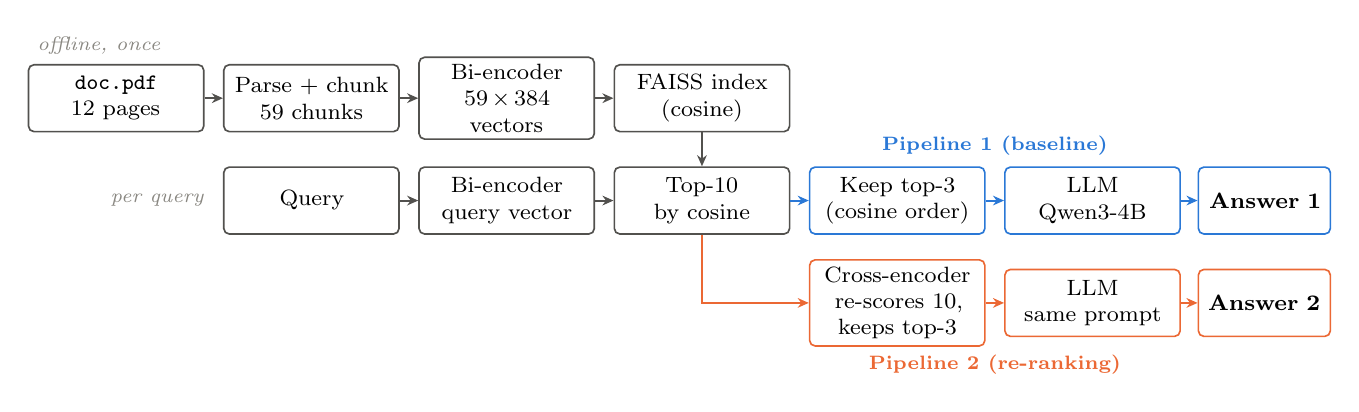
\begin{tikzpicture}[
    font=\footnotesize, >={Stealth[length=4pt,width=3.5pt]},
    box/.style={draw=#1, rounded corners=2pt, line width=0.6pt, align=center,
                text width=2.05cm, inner sep=2.5pt, minimum height=8.5mm, fill=white},
    box/.default=inktwo,
    flow/.style={->, line width=0.7pt, draw=#1}, flow/.default=inktwo,
    lane/.style={font=\scriptsize\itshape, text=muted, anchor=east}]
  \def\dx{2.48}
  % offline indexing
  \node[box] (pdf)   at (0*\dx, 0) {\texttt{doc.pdf}\\12 pages};
  \node[box] (chunk) at (1*\dx, 0) {Parse + chunk\\59 chunks};
  \node[box] (emb)   at (2*\dx, 0) {Bi-encoder\\59\,$\times$\,384 vectors};
  \node[box] (idx)   at (3*\dx, 0) {FAISS index\\(cosine)};
  % per-query, shared first stage
  \node[box] (q)     at (1*\dx, -1.3) {Query};
  \node[box] (qe)    at (2*\dx, -1.3) {Bi-encoder\\query vector};
  \node[box] (top10) at (3*\dx, -1.3) {Top-10\\by cosine};
  % pipeline 1
  \node[box=pone] (p1)  at (4*\dx, -1.3) {Keep top-3\\(cosine order)};
  \node[box=pone] (l1)  at (5*\dx, -1.3) {LLM\\Qwen3-4B};
  \node[box=pone, text width=1.5cm] (a1) at (5.88*\dx, -1.3) {\textbf{Answer 1}};
  % pipeline 2
  \node[box=ptwo] (ce)  at (4*\dx, -2.6) {Cross-encoder\\re-scores 10, keeps top-3};
  \node[box=ptwo] (rs)  at (5*\dx, -2.6) {LLM\\same prompt};
  \node[box=ptwo, text width=1.5cm] (a2) at (5.88*\dx, -2.6) {\textbf{Answer 2}};
  \draw[flow] (pdf) -- (chunk);  \draw[flow] (chunk) -- (emb);  \draw[flow] (emb) -- (idx);
  \draw[flow] (q) -- (qe);       \draw[flow] (qe) -- (top10);   \draw[flow] (idx) -- (top10);
  \draw[flow=pone] (top10) -- (p1); \draw[flow=pone] (p1) -- (l1); \draw[flow=pone] (l1) -- (a1);
  \draw[flow=ptwo] (top10.south) |- (ce.west);
  \draw[flow=ptwo] (ce) -- (rs); \draw[flow=ptwo] (rs) -- (a2);
  % lane labels
  \node[lane, anchor=south west] at (pdf.north west) {offline, once};
  \node[lane] at ($(q.west)+(-0.12,0)$) {per query};
  \node[font=\scriptsize\bfseries, text=pone, anchor=south] at ($(p1.north)!0.5!(l1.north)+(0,0.02)$) {Pipeline 1 (baseline)};
  \node[font=\scriptsize\bfseries, text=ptwo, anchor=north] at ($(ce.south)!0.5!(rs.south)+(0,-0.04)$) {Pipeline 2 (re-ranking)};
\end{tikzpicture}
\caption{The two pipelines share the chunked corpus, the FAISS index and the first-stage top-10.
They differ only in how the three chunks given to the LLM are chosen.}
\label{fig:arch}
\end{figure}
\vspace{-8pt}

% =============================================================================
\section{Architecture comparison}

% TODO: write your answer here, in your own words.

\begin{guide}{Section 1}
the core difference between a bi-encoder (independent embeddings, cosine similarity)
and a cross-encoder (joint self-attention across tokens).
\begin{evidence}
  \item Bi-encoder \nb{4}: the 59 chunks were embedded once into a 59\,$\times$\,384 matrix (0.24\,s);
        each query then needs one encoder pass (4.3\,ms GPU) and a 0.02\,ms FAISS search.
        Cosine scores seen in the top-10 lists: 0.17--0.60. Input limit 256 tokens (chunk 1, 311 tokens, is truncated).
  \item Cross-encoder \nb{5}: nothing is stored; each of the 10 (query, chunk) pairs is one forward pass returning a
        single relevance logit (seen: $-11.4$ to $+7.4$); 9.7\,ms for 10 pairs on GPU.
  \item Both are 6-layer MiniLM models with $\approx$22.7\,M parameters and 384-d hidden states.
\end{evidence}
\end{guide}

% =============================================================================
\section{Qualitative and rank-shift analysis}

\begin{table}[H]
\centering\footnotesize
\caption{Rank of the gold chunk (the chunk that holds the answer) among the 10 bi-encoder candidates, and the
three chunks each pipeline sent to the LLM (gold chunks in bold). Source: \texttt{results/rank\_shifts.csv}.}
\label{tab:ranks}
\begin{tabularx}{\textwidth}{@{}l>{\raggedright\arraybackslash}Xl c c c l l@{}}
\toprule
 & Query & Failure type & Gold & P1 rank & P2 rank & P1 context & P2 context \\
\midrule
F1 & Can I overbuild an opponent's brewery? & Negation / role limit & 43, 53 & \#10 & \#1 & 52, 34, 44 & \gold{43}, 34, 52 \\
F2 & What happens to level 1 industries at the end of the canal era? & Exception & 27 & \#7 & \#1 & 56, 42, 51 & \gold{27}, 55, 26 \\
F3 & Does my income level give victory points at the end of the game? & Keyword trap & 55 & \#6 & \#1 & 24, 57, 30 & \gold{55}, 24, 57 \\
F4 & What happens when the deck runs out of cards? & Synonyms & 21 & \#5 & \#1 & 28, 20, 14 & \gold{21}, 28, 20 \\
F5 & Is the general supply of cubes limited? & Buried chunk & 16 & \#6 & \#3 & 40, 33, 2 & 32, 43, \gold{16} \\
\midrule
L1 & Can my opponent use coal from my mine? & Re-ranker demotes & 31 & \#1 & \#5 & \gold{31}, 32, 52 & 43, 32, 53 \\
L2 & What do I get for selling to Warrington with beer? & First-stage miss & 46 & ${>}10$ & ${>}10$ & 34, 44, 15 & 15, 44, 34 \\
L3 & Can I upgrade a factory to a better one? & Low CE confidence & 42, 43 & \#1 & \#2 & \gold{42}, 55, 51 & 30, \gold{43}, 4 \\
\bottomrule
\end{tabularx}
\end{table}

\begin{figure}[H]
\centering
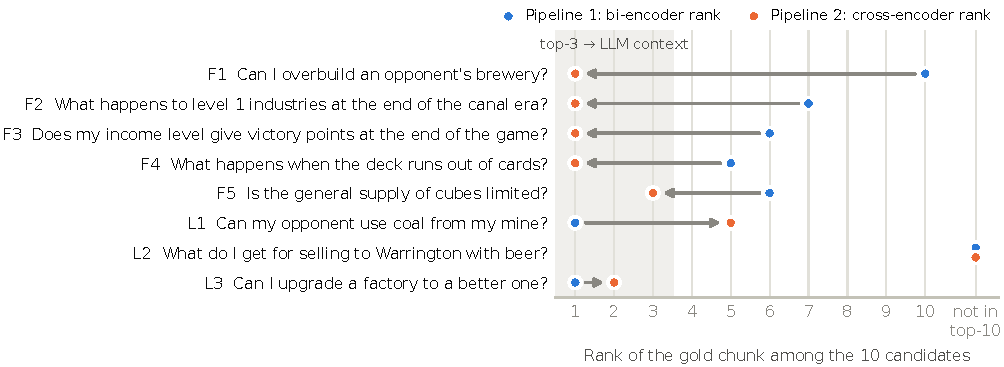
\includegraphics[width=\textwidth]{figures/rank_shifts.pdf}
\caption{Gold-chunk rank under each pipeline. Arrows run from the bi-encoder rank to the cross-encoder rank;
the shaded band is the top-3 passed to the LLM.}
\label{fig:ranks}
\end{figure}

\begin{table}[H]
\centering\footnotesize
\caption{Answer 1 (baseline) vs.\ Answer 2 (re-ranked), excerpted verbatim; full answers in
\texttt{results/answers.csv}. Marks compare each answer with the rulebook:
\ok~correct, \pmark~partly correct, \no~wrong, \abst~declined to answer.}
\label{tab:answers}
\begin{tabularx}{\textwidth}{@{}l
  >{\raggedright\arraybackslash}X
  >{\raggedright\arraybackslash}X
  >{\raggedright\arraybackslash}p{3.3cm}@{}}
\toprule
 & Answer 1 (Pipeline 1) & Answer 2 (Pipeline 2) & Rulebook \\
\midrule
F1 & \abst~\enquote{\dots{} based on the provided excerpts, this question cannot be answered.}
   & \ok~\enquote{No \dots{} Overbuilding is only allowed for opponent-owned Coal Mines or Iron Works.}
   & No: only an opponent's Coal Mine or Iron Works, and only when no such cubes are left. \\
F2 & \no~\enquote{\dots{} level 1 industries remain on the board and can be upgraded or replaced during the Rail Era~\dots}
   & \ok~\enquote{\dots{} all level 1 Industry tiles are removed from the board and returned to the box.}
   & Removed to the box; level 2+ tiles stay. \\
F3 & \ok~\enquote{No \dots{} income level gives victory points only in the introductory game~\dots}
   & \no~\enquote{Yes \dots{} you score VPs equal to your income level~\dots}
   & No; only the introductory game scores income. \\
F4 & \pmark~\enquote{\dots{} rounds continue until both the Draw Deck and players' Hands are exhausted.
     After that, the Rail Era scoring is performed~\dots}
   & \ok~\enquote{\dots{} players' Hands decrease each round until they have no cards left.}
   & Hands shrink each round; the era ends when they are empty. \\
F5 & \no~\enquote{Yes, the general supply of cubes is limited. The rulebook states there are 18 Iron cubes and 30 Coal cubes~\dots}
   & \ok~\enquote{No \dots{} The General Supply is limitless.}
   & No, the General Supply is limitless. \\
\midrule
L1 & \ok~\enquote{Yes \dots{} the closest \dots{} connected unflipped Coal Mine \dots{} (owned by any player).}
   & \no~\enquote{No \dots{} coal from a mine belongs to the owner of that mine.}
   & Yes, from any player's connected Coal Mine. \\
L2 & \no~\enquote{In a 2-player game, no Merchant tiles are placed in Warrington \dots{} you get nothing~\dots}
   & \abst~\enquote{\dots{} the exact reward \dots{} is not specified in the excerpts.}
   & \pounds 5 from the Bank. \\
L3 & \ok~\enquote{Yes \dots{} Overbuilding allows you to replace an already placed Industry tile with a higher-level tile~\dots}
   & \abst~\enquote{The rulebook does not provide information about upgrading a factory~\dots}
   & Yes, by Overbuilding. \\
\bottomrule
\end{tabularx}
\end{table}

\begin{table}[H]
\centering\footnotesize
\caption{Retrieval quality over the 76 labelled questions \nb{9}. Hit@$k$: gold chunk within the top $k$;
MRR@10: mean of 1/rank. Right: where the gold chunk landed relative to the LLM's top-3.}
\label{tab:eval}
\begin{tabular}[t]{@{}lcccc@{}}
\toprule
 & Hit@1 & Hit@3 & MRR@10 & Recall@10 \\
\midrule
Pipeline 1 (bi-encoder)      & 0.605 & 0.816 & 0.724 & 0.947 \\
Pipeline 2 (+ cross-encoder) & \textbf{0.697} & \textbf{0.882} & \textbf{0.794} & 0.947 \\
\bottomrule
\end{tabular}
\hspace{1.2em}
\begin{tabular}[t]{@{}lr@{}}
\toprule
Gold chunk vs.\ top-3 & Questions \\
\midrule
moved \emph{into} top-3 by re-ranking & 8 \\
pushed \emph{out of} top-3 by re-ranking & 3 \\
in top-3 under both / neither & 59 / 6 \\
\bottomrule
\end{tabular}
\end{table}

% TODO: write your answer here, in your own words.

\begin{guide}{Section 2}
document the rank changes for the failure queries, and compare Answer 1 vs.\ Answer 2: did the baseline
hallucinate, omit an essential clause or misstate a rule because the critical chunk sat outside the top 3?
\begin{evidence}
  \item Table~\ref{tab:ranks} / Fig.~\ref{fig:ranks}: every F-case gold chunk starts at rank 5--10 and ends in the top-3; F1 moves furthest (\#10\ra\#1).
  \item Table~\ref{tab:answers}, F1--F5: Answer 1 declines (F1), states the wrong rule (F2), is partly wrong (F4) and invents
        cube counts (F5); in F3 it is Answer 2 that is wrong.
  \item F3: chunk 55 (``income level \dots{} is not worth VPs'') reaches \#1, but chunk 57 (introductory-game scoring) is still in the P2 context.
  \item L1: chunk 31 (coal from a mine ``owned by any player'') drops \#1\ra\#5; the cross-encoder ranks chunk 43 (Overbuilding) and 32 (Coal Market) above it.
  \item L2: chunk 46 (Warrington's \pounds 5 bonus) is in neither top-10, so both pipelines see the same three chunks in a different order.
  \item L3: all ten cross-encoder logits lie between $-10.67$ and $-11.40$; in F1--F3 the top logit is $+3.4$ to $+6.9$.
  \item Table~\ref{tab:eval}: Hit@3 rises 0.816\ra0.882 (8 in, 3 out); Recall@10 is unchanged.
\end{evidence}
\end{guide}

% =============================================================================
\section{Latency profiling}

\begin{table}[H]
\centering\footnotesize
\caption{Left: retrieval latency per query in ms, median (p95), over 76 questions $\times$ 5 repeats \nb{10}.
Right: mean end-to-end latency in ms on the GPU for the eight test queries, models already loaded.
Sources: \texttt{results/latency\_retrieval.csv}, \texttt{latency\_end\_to\_end.csv}.}
\label{tab:latency}
\begin{tabular}[t]{@{}lrr@{}}
\toprule
Stage & GPU & CPU \\
\midrule
Query embedding (bi-encoder)          & 4.26 (6.57)  & 8.21 (8.91) \\
FAISS search, 59 chunks               & 0.02 (0.03)  & 0.03 (0.03) \\
\textcolor{pone}{\textbf{Pipeline 1 retrieval}} & \textbf{4.28} (6.60) & \textbf{8.24} (8.94) \\
Cross-encoder, 10 pairs               & 9.65 (11.61) & 92.03 (115.71) \\
\textcolor{ptwo}{\textbf{Pipeline 2 retrieval}} & \textbf{14.24} (17.74) & \textbf{100.44} (124.75) \\
\midrule
Pipeline 2 / Pipeline 1 (median)      & $\times$3.3 & $\times$12.2 \\
\bottomrule
\end{tabular}
\hspace{1em}
\begin{tabular}[t]{@{}lrr@{}}
\toprule
 & \textcolor{pone}{\textbf{P1}} & \textcolor{ptwo}{\textbf{P2}} \\
\midrule
Retrieval            & 6.0    & 6.0 \\
Re-ranking           & --     & 9.9 \\
LLM generation       & 2288.5 & 2011.1 \\
\textbf{Total}       & \textbf{2294.6} & \textbf{2027.1} \\
\midrule
Answer length (tokens, mean) & 52.8 & 46.0 \\
LLM time per token   & \multicolumn{2}{c}{42--46 ms} \\
\bottomrule
\end{tabular}
\end{table}

% TODO: write your answer here, in your own words.

\begin{guide}{Section 3}
record and tabulate the runtime of the baseline retrieval vs.\ the re-ranking pipeline (Table~\ref{tab:latency}).
\begin{evidence}
  \item Re-ranking adds about 10\,ms per query on the GPU and about 92\,ms on the CPU.
  \item Retrieval as a share of end-to-end time: 6.0/2294.6 = 0.26\,\% (P1) and 15.9/2027.1 = 0.78\,\% (P2).
  \item P2's total is lower here while its answers average 46.0 tokens vs.\ 52.8 for P1, at 42--46\,ms per token.
\end{evidence}
\end{guide}

% =============================================================================
\section{Scaling question}

\begin{figure}[H]
\centering
\begin{minipage}[c]{0.585\textwidth}
  \centering
  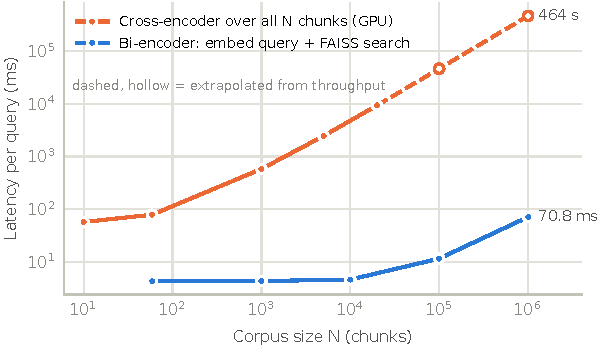
\includegraphics[width=\linewidth]{figures/scaling.pdf}
\end{minipage}\hfill
\begin{minipage}[c]{0.395\textwidth}
  \centering\footnotesize
  \begin{tabular}{@{}rrrr@{}}
  \toprule
  $N$ & Bi-enc.\ + & \multicolumn{2}{c}{Cross-encoder, all $N$} \\
  \cmidrule(l){3-4}
  chunks & FAISS & GPU & CPU \\
  \midrule
  59        & 4.3 ms  & 78 ms     & 0.82 s \\
  1\,000    & 4.3 ms  & 0.58 s    & 8.5 s$^*$ \\
  100\,000  & 11.5 ms & 46 s$^*$  & 14 min$^*$ \\
  1\,000\,000 & 70.8 ms & 7.7 min$^*$ & 2.4 h$^*$ \\
  \bottomrule
  \end{tabular}\\[4pt]
  \parbox{\linewidth}{\scriptsize $^*$\,extrapolated from the measured throughput: 2\,156 pairs/s (GPU),
  118 pairs/s (CPU). One-off bi-encoder indexing: 0.55\,ms per chunk, ${\approx}9.2$\,min for 1\,M chunks.}
\end{minipage}
\caption{Cost of one query as the collection grows \nb{11}. Bi-encoder side: embed the query, then exact FAISS search over $N$
vectors (random unit vectors stand in for $N > 59$). Cross-encoder side: score every (query, chunk) pair, as a
cross-encoder-only system would. Sources: \texttt{results/scaling\_*.csv}.}
\label{fig:scaling}
\end{figure}

% TODO: write your answer here, in your own words.

\begin{guide}{Section 4}
why we do not simply run a cross-encoder across the entire document collection from the very start.
\begin{evidence}
  \item Fig.~\ref{fig:scaling}: per-query cross-encoder cost grows linearly with $N$ (7.7\,min per query on GPU and 2.4\,h on CPU at 1\,M chunks),
        against 70.8\,ms for query embedding + exact FAISS search.
  \item The bi-encoder's chunk vectors cost 0.55\,ms per chunk, paid once at indexing time; Table~\ref{tab:latency} shows the per-query part.
  \item For this 59-chunk rulebook, scoring every chunk takes 78\,ms on GPU.
  \item First-stage Recall@10 = 0.947 (Table~\ref{tab:eval}): the share of questions whose gold chunk reaches the re-ranker at all.
\end{evidence}
\end{guide}

\end{document}
